\chapter{Design}
\label{chap:design}

\section{Introduction}
\label{sec:designintroduction}

The goal of this thesis is to develop a modularized and production grade user simulator that can be re-targeted for new domains and provide a framework to produce training data and train dialog agents. The overall design for the simulator was inspired by the work done by \cite{li_usersim} and the formalization of hidden user agenda models by \cite{Schatzmann2009TheHA}. 

Underlying the simulator is a framework that consists the following components:
\begin{itemize}
	\item \textbf{User Simulator}: An agenda based user modeling component that generates natural language speech utterances to simulate what an actual human would say in the context of task-completion dialog activity. 
	\item \textbf{Dialog Agent API}: A set of methods to allow a researcher to provide an agent(s) that simulate how the system / dialog agent would respond 
	\item \textbf{Dialog Manager}: A coordinator component that tracks the current state of the dialog and facilitates the conversation between the user simulator and dialog agent/system. Add the end of the simulated conversation, the manager will evaluate and score the conversion. 
\end{itemize}

Note, we defer discussing the implementation details until the Implementation chapter (Chapter~\ref{chap:implementation}).

\section{User Simulator} 

The user simulator is responsible for imitating a real user and generating realistic speech utterances. Here we assume the user is an actor that is attempting complete task. For example, the user may want to travel to Japan and is attempting to book a flight there. That user could then interact with a travel agent chatbot in order to get assistance in identifying the appropriate flight and purchasing tickets. In order to model and represent a user, we will utilize the formalization of the hidden user agenda described in \cite{Schatzmann2009TheHA}.

 One of the primary assumptions here is that user has intentionally engaged with the dialog agent in order to complete their task. At the outset of the conversation, the user will have some specific goal in mind (order Indian food, book a flight to Japan, etc). The dialog agent will attempt to learn user's goal by asking the user a set of clarifying questions. Schatzmann introduces the idea of a hidden user agenda as a mechanism to represent the sequence of dialog acts and utterances a user will say in the context of that conversation. At each step of a task-completion dialog, the user is either responding to the dialog agent or initiating a new conversation direction. The user agenda provides an efficient way and formal structure to represent the pending set of dialog acts the user will communicate to the dialog agent.
 
Socrates Simulator implements the Schatzmann's concept of user agenda and user goal as first class objects. The conversion from the formal representation to code is rather straightforward as there are analogous data structures. We will defer discussing implementation details until the next chapter. The subsections below will further describe how the user goal and agenda is defined. 

\subsection{User Goals} 
The user goal captures explicitly both user's preferences and missing information needs they are trying to fill. For example, take a user who wants to find an Indian restaurant in Central square for dinner. We can decompose this goal into two distinct components. The first is the user's explicit preferences. In this example, their preferred cuisine is Indian. The second component is implicit and unknown to the user. They are looking for a restaurant or more specifically the name and presumably the restaurant's phone number and address. This information is unknown but can be broken down into discrete pieces of information the user will attempt to elicit from the dialog agent as a request for more information. 

Formally, Schatzmann defines the user goal \textit{G} as \textit{G = (C,R)}, where \textit{C} consists of constraints or the user's explicit preferences and \textit{R} represents the user's requests. The constraints and requests are explicitly represented as slot-value pairs. \ref{fig:goals1} below shows how one could represent the goal of user looking for a bar. 

\begin{figure}[h!]
	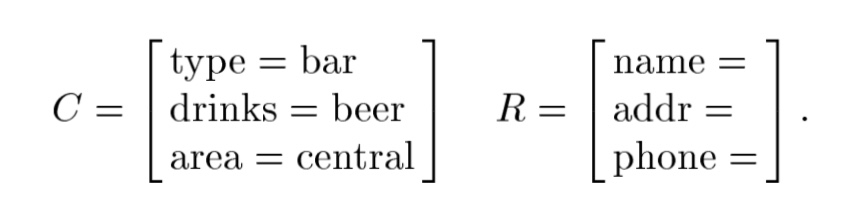
\includegraphics[width=\linewidth]{diagrams/schatzmann_goal_fig.jpeg}
	\caption{Example User goal. User wants the name, address and phone number of a cheap bar in central.  }
	\label{fig:goals1}
\end{figure}

The concept of a goal abstractly turns out to be useful in also driving the dialog manager's simulations. We abstract the idea of goal and make it available to both the user and dialog agent api as way to track the internal state of each speaker. 

\subsection{User Agenda} 







\section{Dialog Model Overview}

\subsection{Speaker}
\subsection{Goals}
\subsection{Dialog Status}
\subsection{Dialog Acts}
\subsection{Natural Language Understanding}
\subsection{Natural Language Generation}


\section{Reinforcement Learning Support}
tbd
\subsection{Replay Conversation}
tbd
\subsection{Reward Function}
tbd

%%% Local Variables: 
%%% mode: latex
%%% TeX-master: "main"
%%% End: 
